\chapter{Cloud Encryption}


\section{Cloud computing}
Cloud computing is defined as using remote, Internet-based servers for computational or storage resources. This has some pros and cons: first it is accessible from anywhere, any time and maintenance done by someone else (unless self-hosted!), it's cost-effective, as part of a shared data-center and it has scalable resources, on the other side availability relies on Internet connection and server reliability, long-distance communication creates a performance hit and your data is on someone else’s machines.

Services are provided by third parties and not in house, users have no real guarantee that the cloud service providers are doing what they claim to be doing: trust becomes a key issue. The main security problem with cloud computing is that data loaded into the cloud is no longer in the control of the data creator/data controller and cloud service providers may be honest but curious.

When the data has to be retrieved, processed or searched, use of standard encryption is not useful: one has: either to allow the cloud to decrypt the data (this needs trust in cloud service providers) or to download the entire data set to the user’s machine (this spoils the benefits of moving to the cloud in the first place). Even if processing is not required, one needs some additional cryptographic functionality to be able to search and retrieve data which has been stored (encrypted) in the cloud. One of the advantages of using the cloud is the possibility to use well-engineered and managed security services, it is typically still the responsibility of customers to configure such services appropriately (split/shared responsibility model).

\subsection{Fully homomorphic encryption (FHE)}
An arithmetic circuit can be applied to a ciphertext and the result is the encryption of the output of the arithmetic circuit as if it had been evaluated on the underlying plaintext. 
Data owners encrypt their data $\mathcal{D}$, to obtain $enc(\mathcal{\mathcal{D}})$ and send it to the cloud provider. Then suppose the data owners wanted to perform some operation $f$ on the data  to obtain $f(\mathcal{D})$ (for example search). The cloud can compute $enc(f(\mathcal{D}))$ which is then returned to the data owners, the data owners then decrypt this ciphertext to obtain $f(\mathcal{D})$. The main problem is efficiency and scalability.
Each operation on the ciphertext results in compounding noise.
But it results in loss of homomorphic property after a certain number of operations. Also the combination of the noise production followed by the noise reduction makes the scheme completely impractical: in order to perform one search on Google using this encryption, the amount of computations needed would increase by a trillion.

\subsection{Somewhat homomorphic encryption}
The scheme can do both addition and multiplication to the original plaintexts but its capability is heavily limited. For example, it is possible to perform unlimited additions but only one level of multiplication to the ciphertext.

\subsection{Partial homomorphic encryption}
Partial homomorphic encryption: Homomorphism property only with respect to some operations and not others. For example if homomorphic with respect to addition (multiplication), it is not possible to compute multiplications (additions, respectively) over ciphertexts.


\subsection{Multi-party computation (MPC)}
It allows the equivalent of FHE with the use of multiple servers as opposed to a single one. Thus data can be securely outsourced to multiple cloud providers who then can compute on this data, such that one can tolerate a set of colluding adversaries (up to some bound on the number).

Data owners split their data $\mathcal{D}$ into chunks $\mathcal{D}_1 ,\ldots, \mathcal{D}_n$ via a secret sharing scheme. The shares are then distributed to $n$ distinct cloud providers. The cloud providers are now able to compute any function $f(\mathcal{D})$, but they obtain partial results (called shares) that are then returned to the data owners for combining into the final solution $f(\mathcal{D})$ (computing shares may require some exchange of information among providers). As long as the data owners trust $n - t$ out of the $n$ providers, their data is still kept confidentially where $t$ is the maximum number of adversaries which can be tolerated.

\subsection{Searchable encryption}
Solve the following problem: a user outsources a database to a server and then wants to query the server to obtain data. Question: what does security mean in this context? The database contents should remain private to the client and in some cases also the access patterns should be private. Two variants: public or symmetric key. In both variants, the encrypted database is augmented with a set of tokens. Each token is associated with a keyword. The database is encrypted with any encryption algorithm, the searchable encryption scheme is solely used to construct and search for the tokens. Public key variant is vulnerable to selected keywords attack and thus is less adopted. Symmetric key variant is combined with Oblivious RAM techniques to guarantee also the privacy of access patterns. 
A server, which maintains a data storage system, can gain information about its users’ habits and interests, and violate their privacy, even without being able to decrypt the data that they store. The server can monitor the queries made by the clients and perform different traffic analysis tasks. It can learn the usual pattern of accessing the encrypted data, and try to relate it to other information it might have about the clients.
For example, if a sequence of queries $q_1, q_2, q_3$ is always followed by a stock-exchange action, a curious server can learn about the content of these queries, even though they are encrypted, and predict the user action when the same (or similar) sequence of queries appears again. Moreover, it is possible to analyze the importance of different areas in the database, e.g., by counting the frequency of the client accessing the same data items. If the server is an adversary with significant but limited power, it can concentrate its resources in trying to decrypt only data items which are often accessed by the target-user.

\subsection{Order preserving encryption}
It solves a variant of the searchable encryption problem in another way. It enables ciphertexts to be ordered in a way which respects the ordering of the underlying plaintexts. Thus binary search can be conducted on the ciphertexts. The key problem is that the security properties are very weak.

\subsection{Attribute based encryption}

It extends Identity Based Encryption where decryption of data is allowed on the basis of whether the decryptor satisfies a set of policies associated with given secret keys, which in turn are associated to attributes. Complex access control policies for encrypted outsourced data can be embedded within the ciphertext itself. This means that a data owner does not need to trust the cloud provider to implement a policy they require \ref{fig:attributebased}.

\begin{figure}
	\centering
	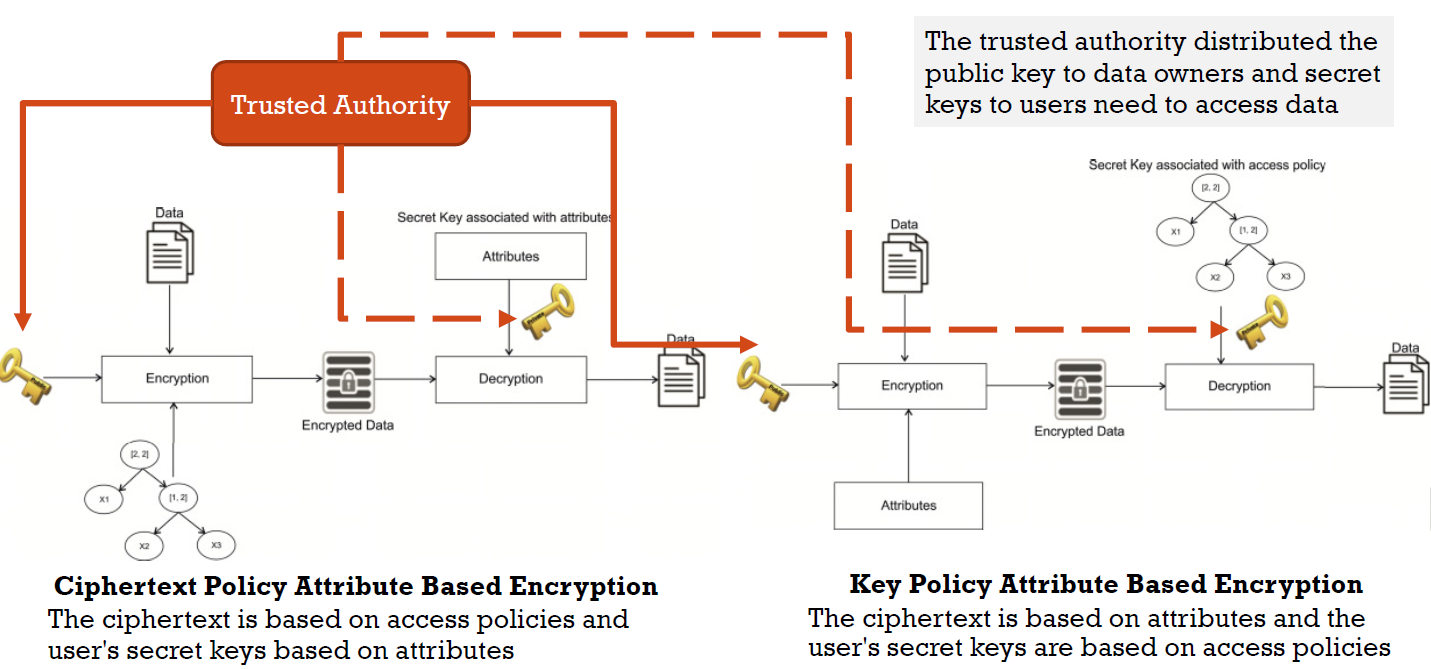
\includegraphics[width=0.7\linewidth]{Images/Chapter8/attribute_based}
	\caption{}
	\label{fig:attributebased}
\end{figure}

Identity-based encryption is a type of public-key encryption in which a user can generate a public key from a known unique identifier such as an email address and a trusted third-party server calculates the corresponding private key from the public key. In this way, there is no need to distribute public keys ahead of exchanging encrypted data. The sender can simply use the unique identifier of the receiver to generate a public key and encrypt the data. The receiver can generate the corresponding private key with the help of the trusted third-party server.

\subsection{Delegated computation}
A resource constrained client can delegate a computation to a powerful service provider. The client can check whether the provider has performed the correct computation. Two running modes, in the non-private mode cloud server learns the clients data, in the private mode the input data, and perhaps the function, are kept private. Theoretical results that combine techniques from FHE, ABE, and MPC.


\subsection{Maturity levels}

Maturity levels in picture \ref{fig:maturitylevels}.

\begin{figure}
	\centering
	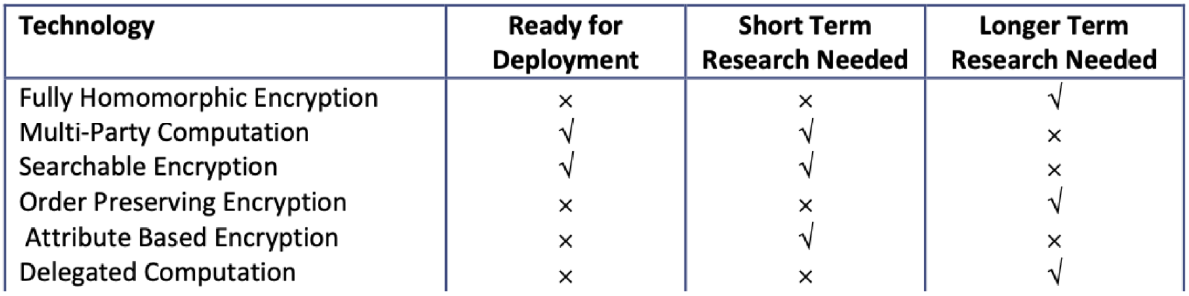
\includegraphics[width=0.7\linewidth]{Images/Chapter8/maturity_levels}
	\caption{Maturity levels}
	\label{fig:maturitylevels}
\end{figure}

\section{Cloud storage}

Essentially your data/files are stored on a remote server and we have conflicting requirements: need to keep data confidential with respect to the curious but honest cloud service provider and support controlled sharing of data, i.e. employees should be able to selectively access data stored in files to be able to perform their jobs. Use cryptography to enforce access control policies so that sharing among employees is permitted while protecting against curious service providers. Role based access control uses role hierarchies to make the specification of policies more compact. These can always be compiled away without loss of generality. We have two tables: UA: user-role assignment, PA: permission-role assignment. User $u$ has permission $p$ iff there exists role $r$ such that $(u,r)$ in UA and $(r,p)$ in PA \ref{fig:cloudstorage}.

\begin{figure}
	\centering
	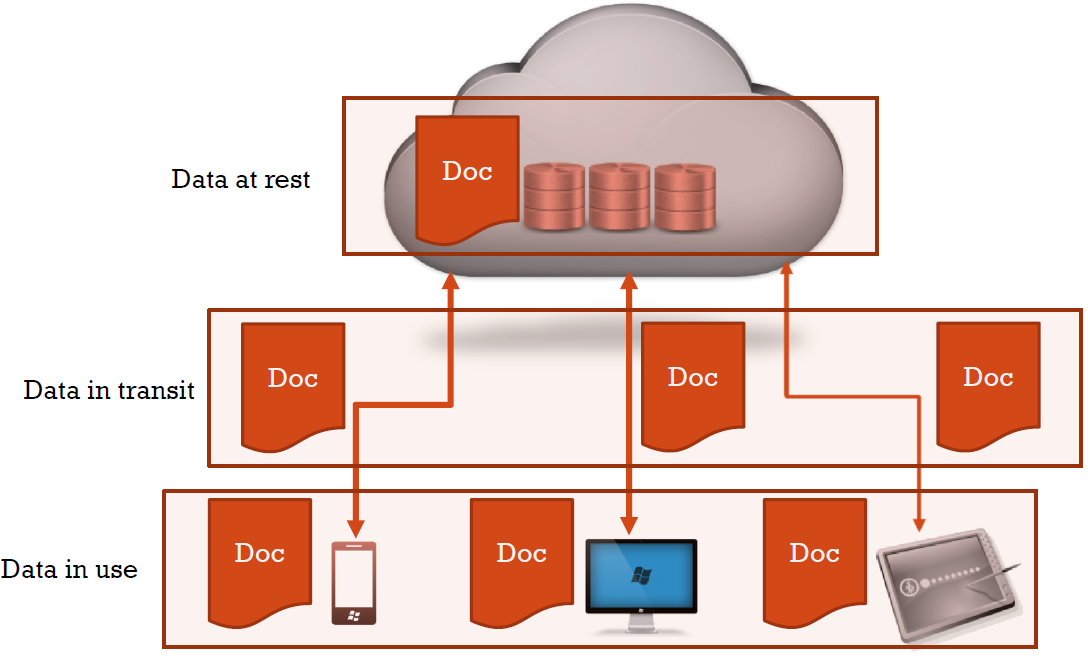
\includegraphics[width=0.7\linewidth]{Images/Chapter8/cloud_storage}
	\caption{Cloud storage}
	\label{fig:cloudstorage}
\end{figure}

\subsection{Hybrid cryptography}

Each user $u$ is equipped with a pair of private and public key: $(ks(u),kp(u))$. Each role $r$ is equipped with a pair of private and public key: $(ks(r),kp(r))$. Each file $f$ is encrypted with a unique symmetric key: $k(f)$. If $(u,r)$ in UA, then compute $\{ks(r)\}kp(u)$ i.e. encrypt the secret key $ks(r)$ associated to $r$ with the public key $kp(u)$ associated to $u$. In this way, $u$ will be able to retrieve the secret key associated to the role by using its private key. If $(r, (read,f))$ in PA, then compute $\{k(f)\}kp(r)$ i.e. encrypt the symmetric key $k(f)$ associated to the file $f$ with the public key of the role $r$.  In this way, a user $u$ with read permission on $f$ (i.e. such that $(u,r)$ in UA and $(r,(read,f))$ in $PA)$ will be able to retrieve the symmetric key associated to $f$ by first retrieving the secret key $ks(r)$ associated to the role which can then be used to retrieve the symmetric key of the file $f$ which is encrypted with the public key $kp(r)$ associated to $r$ \ref{fig:hybridcrypto}.

\begin{figure}
	\centering
	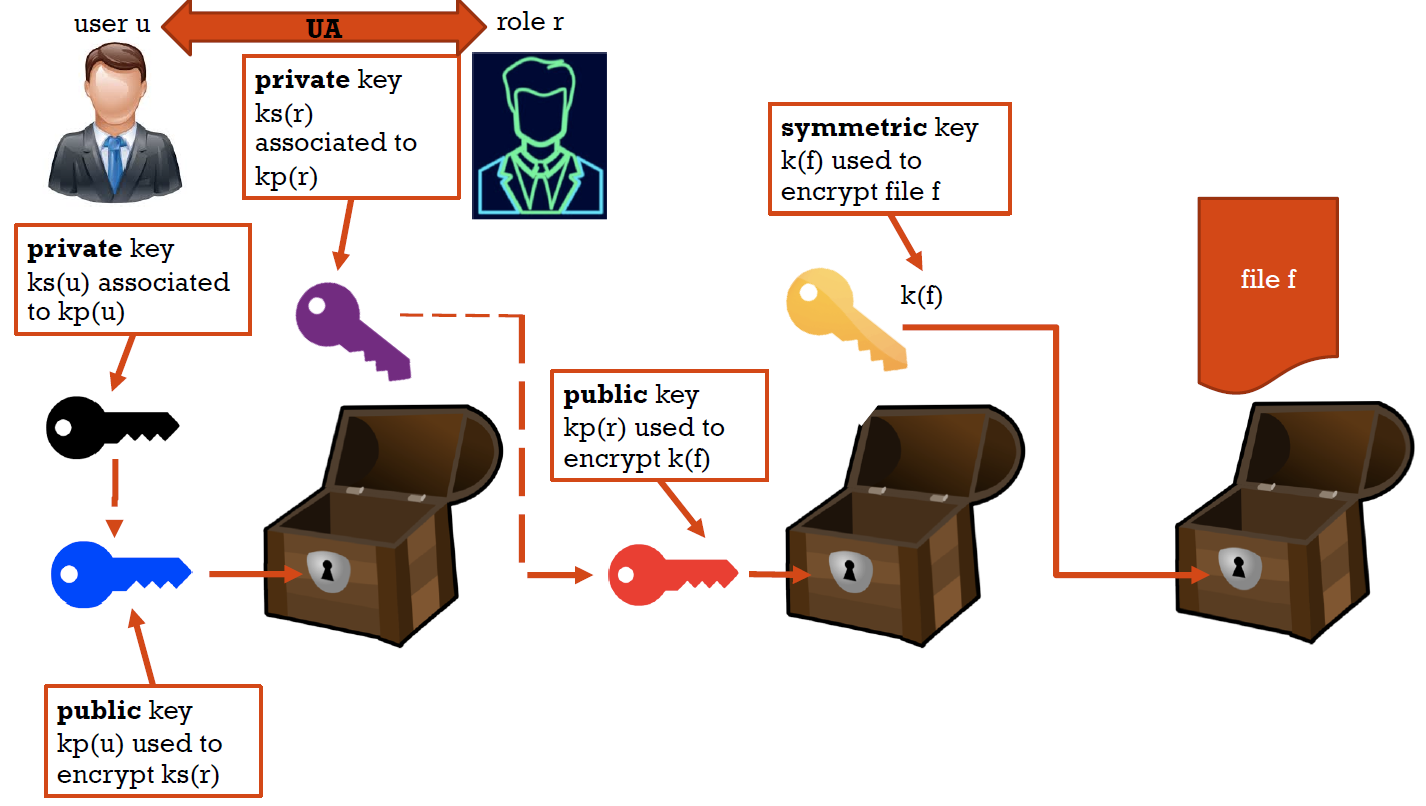
\includegraphics[width=0.7\linewidth]{Images/Chapter8/hybrid_crypto}
	\caption{Hybrid Cryptography}
	\label{fig:hybridcrypto}
\end{figure}

Notice that further auxiliary data (e.g., files version numbers and digital signatures), together referred to as metadata, are needed to enforce policies. Users store their private keys in secure personal devices (e.g., laptops provided with an antivirus) access to which is protected through passwords or similar authentication techniques. Both encrypted data and metadata are stored in the cloud or in a secure area within the organization. To write on a file $f$, a user performs the same operations to obtain the symmetric key $k(f)$ which is used to encrypt the new file. An entity (usually called Reference Monitor) checks whether the user has actually write permission before accepting the new file and storing it in the cloud.

\section{Database-as-a-service (DBaas)}

Not explained \footnote{TODO: Slide 27..31 12-Cloud\_Encryption-2p.pdf}.


\section{Order preserving encryption (OPE)}

Not explained \footnote{TODO: Slide 37..42 12-Cloud\_Encryption-2p.pdf}.


\section{Homomorphic preserving encryption}

Not explained \footnote{TODO: Slide 43..49 12-Cloud\_Encryption-2p.pdf}.

\section{Partially homomorphic}

Homomorphic with respect to multiplication: RSA (1978). Fix a large number $n=p*q$ where $p$ and $q$ are large primes. Find pair of numbers $(e,d)$ such that $e*d \equiv 1 \bmod \phi(n)$. Set $(e,n)$ to be the public key and $(d,n)$ the private key $Enc(m) = m^e \bmod n$. Multiplicative Homomorphism property:
\[Enc(m_1) * Enc(m_2) = m_1 ^ e * m_2 ^ e \bmod N = (m_1 * m_2)^ e \bmod N\]

A scheme is based on the notion of pairing. The advantage of pairing is that it allows us to check if the value of r is equal to the product of a and b. This can be done as follows: given $g^r, g^a, g^b$ checking if $e(g^a,g^b) = e(g^r, g^1)$ is equivalent to $g^{a*b} = g^r$. 

It is possible to combine additive homomorphic scheme with pairing in such a way to compute both the addition and multiplication of the exponents in the group. However, only a limited number of multiplications can be performed as the group on which pairing is applied may generate a group that does not satisfy the conditions for both the additive homomorphic scheme and the pairing.

By simply multiplying two ciphertexts together, one obtains the encryption of the product of the original plaintexts.
Fully homomorphic means we can accommodate any function, but RSA is only homomorphic to multiplication. Pallier is homomorphic to addition but not multiplication.


\section{Full homomorphic encryption}
It centers around a function which introduces a certain level of noise into the encryption. Each operation on the ciphertext results in compounding noise. The noise is resolved with the bootstrapability of the encryption.

\section{Multi party computation for homomorphic encryption}

Not explained \footnote{TODO: Slide 58..60 12-Cloud\_Encryption-2p.pdf}.
